\documentclass[10pt,a4j]{ujarticle} % upLaTeX: ujarticle, pLaTeX: jarticle
\西暦
\usepackage{graphicx}
\usepackage{url}
\usepackage{listings,jlisting}
\usepackage{ascmac}
\usepackage{amsmath,amssymb}

%ここからソースコードの表示に関する設定
\lstset{
  basicstyle={\ttfamily},
  identifierstyle={\small},
  commentstyle={\smallitshape},
  keywordstyle={\small\bfseries},
  ndkeywordstyle={\small},
  stringstyle={\small\ttfamily},
  frame={tb},
  breaklines=true,
  columns=[l]{fullflexible},
  numbers=left,
  xrightmargin=0zw,
  xleftmargin=3zw,
  numberstyle={\scriptsize},
  stepnumber=1,
  numbersep=1zw,
  lineskip=-0.5ex
}
%ここまでソースコードの表示に関する設定

\title{プログラミング応用(知能処理)レポート}
\author{
 3X11XXXX 名工 光/チーム名(チーム番号)\\
}
\date{\today}


\begin{document}
\maketitle

\begin{table}[h]
\center
\caption{相互評価}
\begin{tabular}{l|r}
氏名 & 作業割合 (\%) \\
\hline \hline
A氏 & 50\\
B氏(自分)& 50
\end{tabular}
\vspace{1ex}
\\
{\small 作業全体を100としたときの,各メンバの作業量を申告すること.\\
自分の主観を正直に報告すること.グループ内で調整してはならない.}
\end{table}

\paragraph{全体的な自己評価/作業時間: } A/19.5時間

自己評価を S, A, B, C, D から選択する.作業時間は,成績に影響しないので正直に書くこと.

\paragraph{評価の理由: } calcFiboSeqを実装するにあたり,XXXがYYYになるような独自の手法を工夫した.また,考案した独自手法がどうしてZZZのときにうまくいかないのかを考察し,改善策のアイデアまで示せたので.

\paragraph{全体的な考察: } フィボナッチ数の一般項を実現するにはXXXが重要である点に気がついた.
最初はXXXと予想していたが,実際にプログラムを作成するとYYYという結果になった.解決のためにZZZという工夫をしたところ,評価実験で示したように 100 \% 性能が改善した.最初はXXXと予想していたが,実際にプログラムを作成するとYYYという結果になった.解決のためにZZZという工夫をしたところ,評価実験で示したように 100 \% 性能が改善した.今回,フィボナッチ数をもとめるためのクラス Fibonacci を実装し,インスタンスメソッドとして機能を実装したが,これは静的クラスまたはシングルトンとして実装した方が適していたように考えられる.なぜなら・・・

また,calcFiboメソッドを再帰関数として実装するのではなく,イテレータを用いて実装した場合を考える.イテレータで実装した場合は,実行速度が・・・

calcFiboSeq を実装するにあたり,XXXがYYYになるようにするためにXXXXに着目したが,ZZZのときに処理が失敗するという問題が発生した.これは,ZZZがXXXに対応していないことが原因と考えられる.よって,ZZZを...することで改善できる可能性がある.

\paragraph{全体的な感想: } フィボナッチ数の一般項をもとめるのに夢中であやうく実装が間に合わなくなるところだった.実装に関しては,・・・

%%%%%%%%%%%%%%%%%%%%%%%%%%%%%%%%%%%%%%%%
\section{概要}
\begin{screen}
\begin{enumerate}
\setlength{\itemsep}{2pt}      %2. ブロック間の余白
\setlength{\parskip}{0pt}      %4. 段落間余白.
\item プレイヤ名: {\verb+24XX+}
\item 大会成績: 1位, 999勝0敗1引分け
\item グループ内での作業分担状況の概要: AはXを担当し,BはYを担当した.
\item 自分の担当範囲と簡潔なアピール: 高速化を担当し k 倍の高速化を実現した.
\end{enumerate}
\end{screen}

%%%%%%%%%%%%%%%%%%%%%%%%%%%%%%%%%%%%%%%%
\section{プレイヤについて}

\subsection{使用した探索アルゴリズムとその工夫点}

\begin{lstlisting}[caption=calcFiboメソッドの工夫点,label=src:calcFibo]
    // n番目のフィボナッチ数を計算して返す
    int calcFibo(int n) {
	if (n <= 1) {
	    return 1;
	}
	return calcFibo(n - 1) + calcFibo(n - 2);
    }
\end{lstlisting}

\subsection{評価関数とその工夫点}

\begin{figure}[!hbt]
  \centering
  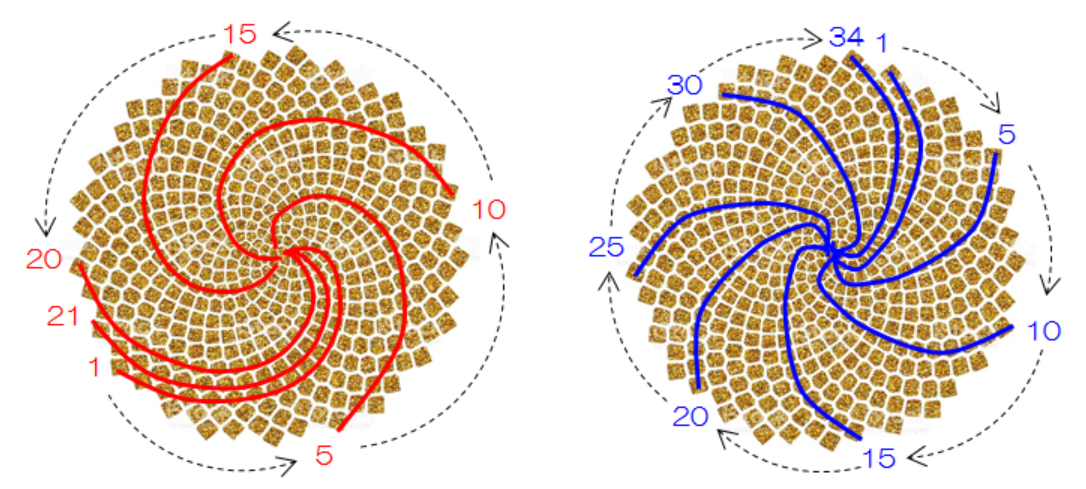
\includegraphics[bb=0 0 782 352,width=0.3\linewidth]{himawari.png}
  \caption{ひまわりの種の並び方}
  \label{fig:himawari}
\end{figure}

\begin{lstlisting}[caption=calcFiboメソッドの工夫点,label=src:calcFibo]
    // n番目のフィボナッチ数を計算して返す
    int calcFibo(int n) {
	if (n <= 1) {
	    return 1;
	}
	return calcFibo(n - 1) + calcFibo(n - 2);
    }
\end{lstlisting}


\subsection{高速化とその工夫点}
\begin{lstlisting}[caption=calcFiboメソッドの工夫点,label=src:calcFibo]
    // n番目のフィボナッチ数を計算して返す
    int calcFibo(int n) {
	if (n <= 1) {
	    return 1;
	}
	return calcFibo(n - 1) + calcFibo(n - 2);
    }
\end{lstlisting}


\subsection{実行速度}(1秒あたりの訪問ノード数)


\subsection{その他の工夫点}


%%%%%%%%%%%%%%%%%%%%%%%%%%%%%%%%%%%%%%%%
\section{考察}

\subsection{実績に期待通りの好影響を与えた工夫点}


\subsection{実績に期待ほどの好影響を与えられなかった工夫点}


\subsection{実績に期待外れの悪影響を及ぼした工夫点}


\subsection{今後の課題}


%%%%%%%%%%%%%%%%%%%%%%%%%%%%%%%%%%%%%%%%
\section{課題}
%%%%%%%%%%%%%%%%%%%%%%%%%%%%%%%%%%%%%%%%
\subsection{課題1}
%%%%%%%%%%%%%%%%%%%%%%%%%%%%%%%%%%%%%%%%
課題1に関する気づきや考察があれば記載する.

%%%%%%%%%%%%%%%%%%%%%%%%%%%%%%%%%%%%%%%%
\subsection{課題2}
%%%%%%%%%%%%%%%%%%%%%%%%%%%%%%%%%%%%%%%%
課題2に関する気づきや考察があれば記載する.

%%%%%%%%%%%%%%%%%%%%%%%%%%%%%%%%%%%%%%%%
\subsection{課題3}
%%%%%%%%%%%%%%%%%%%%%%%%%%%%%%%%%%%%%%%%
課題3に関する気づきや考察があれば記載する.

\section{参考文献・謝辞}
参考にした資料の一覧や,協力者への謝辞を書く.



\end{document}
